\section{Paper 4: Are the patients who would benefit from thrombolysis the same ones as those receiving it? A machine learning study of the UK stroke registry.\cite{pearn_are_2024}}\label{sec:paper_4}

\subsection{Objective}

To investigate, using explainable machine learning, the overlap and differences between the groups of patients receiving thrombolysis, and the group of patients predicted to benefit from thrombolysis.

\subsection{Methods overview}

\subsubsection{Outcome prediction}

Data for a total of 78,396 ischaemic stroke patients who attended one of 111 emergency stroke hospitals in England and Wales and had brain imaging within 255 minutes of stroke onset, from 2016 to 2021, were extracted from the Sentinel Stroke National Audit Programme (SSNAP). We used explainable machine learning (XGBoost\cite{chen_xgboost_2016} with SHAP\cite{lundberg_unified_2017}) to examine the effect of patient characteristics, hospital attended, and use/time of thrombolysis on the patients’ predicted outcome (modified Rankin Scale, mRS) at discharge. Patients on anticoagulants for atrial fibillation (representing 12.9\% of the population) were excluded from the study population as these patients may be at risk of adverse outcome that is not predicted by the machine learning model (as it is likely thrombolysis is only given to patients on anticoagulants when it is sure blood clotting is sufficient).

The model predicts probability of each mRS category outcome.  \textit{Probability-weighted mRS} was used as a measure of the mid-point location of disability; it is the sum of each mRS outcome multiplied by the probability of that outcome occurring

We predicted the expected effect of thrombolysis for all patients, and compared who would benefit from thrombolysis with those who actually received thrombolysis. We used a conservative definition to determine whether a patient would likely have a better outcome with treatment from the two probability distributions, where both of these criteria must be met: 

\begin{enumerate}
    \item A reduction in probability-weighted mRS.
    \item A reduction in the likelihood of a very bad outcome (mRS 5-6, complete dependency or death).
\end{enumerate}

\subsubsection{Hospital trade-off between maximising benefit from thrombolysis and minimising risk of harm from thrombolysis}

We trained a second XGBoost \textit{thrombolysis decision} model, to predict the likelihood of a patient receiving thrombolysis, using methods previously described \cite{pearn_what_2023}. We used this to predict likely thrombolysis use for all patients at all stroke teams. This was used to compare likely decision-making and outcomes across if all stroke teams saw the same patients. To compare maximising benefit from thrombolysis and avoiding potential harm from thrombolysis we defined measures for \textit{sensitivity} and \textit{specificity} of treatment. \textit{Sensitivity} was calculated as the proportion of patients who were predicted to benefit from thrombolysis (from the \textit{thrombolysis outcome} model) who were predicted to receive thrombolysis at each team (from the \textit{thrombolysis decision} model). \textit{Specificity} was calculated as the proportion of patients who were predicted not to benefit from thrombolysis (from the \textit{thrombolysis outcome} model) who were not predicted to receive thrombolysis at each team (from the \textit{thrombolysis decision} model). A low \textit{sensitivity} would indicate a higher likelihood of not treating people who would benefit from thrombolysis, and a low \textit{specificity} would indicate a higher likelihood of treating people who would not benefit from thrombolysis.

Code, and full results, for the machine learning work may be found at \url{https://github.com/samuel-book/thrombolysis_outcome_ml_paper}.

\subsection{Key results}

\subsubsection{Model accuracy}

Receiver Operating Characteristic Area Under Curve (ROC-AUC) was 0.796 (0.001 standard deviation across the 5 k-folds). Classification accuracy across the seven mRS outcomes was 41.1\% (0.002 standard deviation across the 5 k-folds). Accuracy to within one mRS category was 72.4\% (0.002 standard deviation across the 5 k-folds).  

\subsection{Comparing actual use of thrombolysis and predicted benefit from thrombolysis}

We used the first k-fold train/test set split (4:1 train:test data) to investigate likely outcome from thrombolysis. In the test set of 15,680 patients, 44\% received thrombolysis. For each patient we predicted outcomes with and without thrombolysis. Figure \ref{fig:scatter_all} shows the expected shift in probability-weighted mRS at discharge, and the change in probability of being discharged with mRS 5-6, due to thrombolysis, separated by whether the patient actually received thrombolysis or not. Overall, 60\% of patients were predicted to benefit from thrombolysis. Of those who did receive thrombolysis, 73\% were predicted to have both a better average disability likelihood and a reduction in probability of being mRS 5-6. 9\% were predicted to have both a worse average disability likelihood and an increase in probability of being mRS 5-6. 18\% were predicted to have either, but not both, an improved average disability likelihood or a reduction in probability of being mRS 5-6. Of those who did not receive thrombolysis, 49\% were predicted to have both a better average disability likelihood and a reduction in probability of being mRS 5-6. 26\% were predicted to have both a worse average disability likelihood and an increase in probability of being mRS 5-6. 25\% were predicted to have either, but not both, an improved average disability likelihood or a reduction in probability of being mRS 5-6.

\begin{figure}
\centering
\begin{subfigure}{.7\textwidth}
  \centering
  \captionsetup{width=.9\linewidth}
  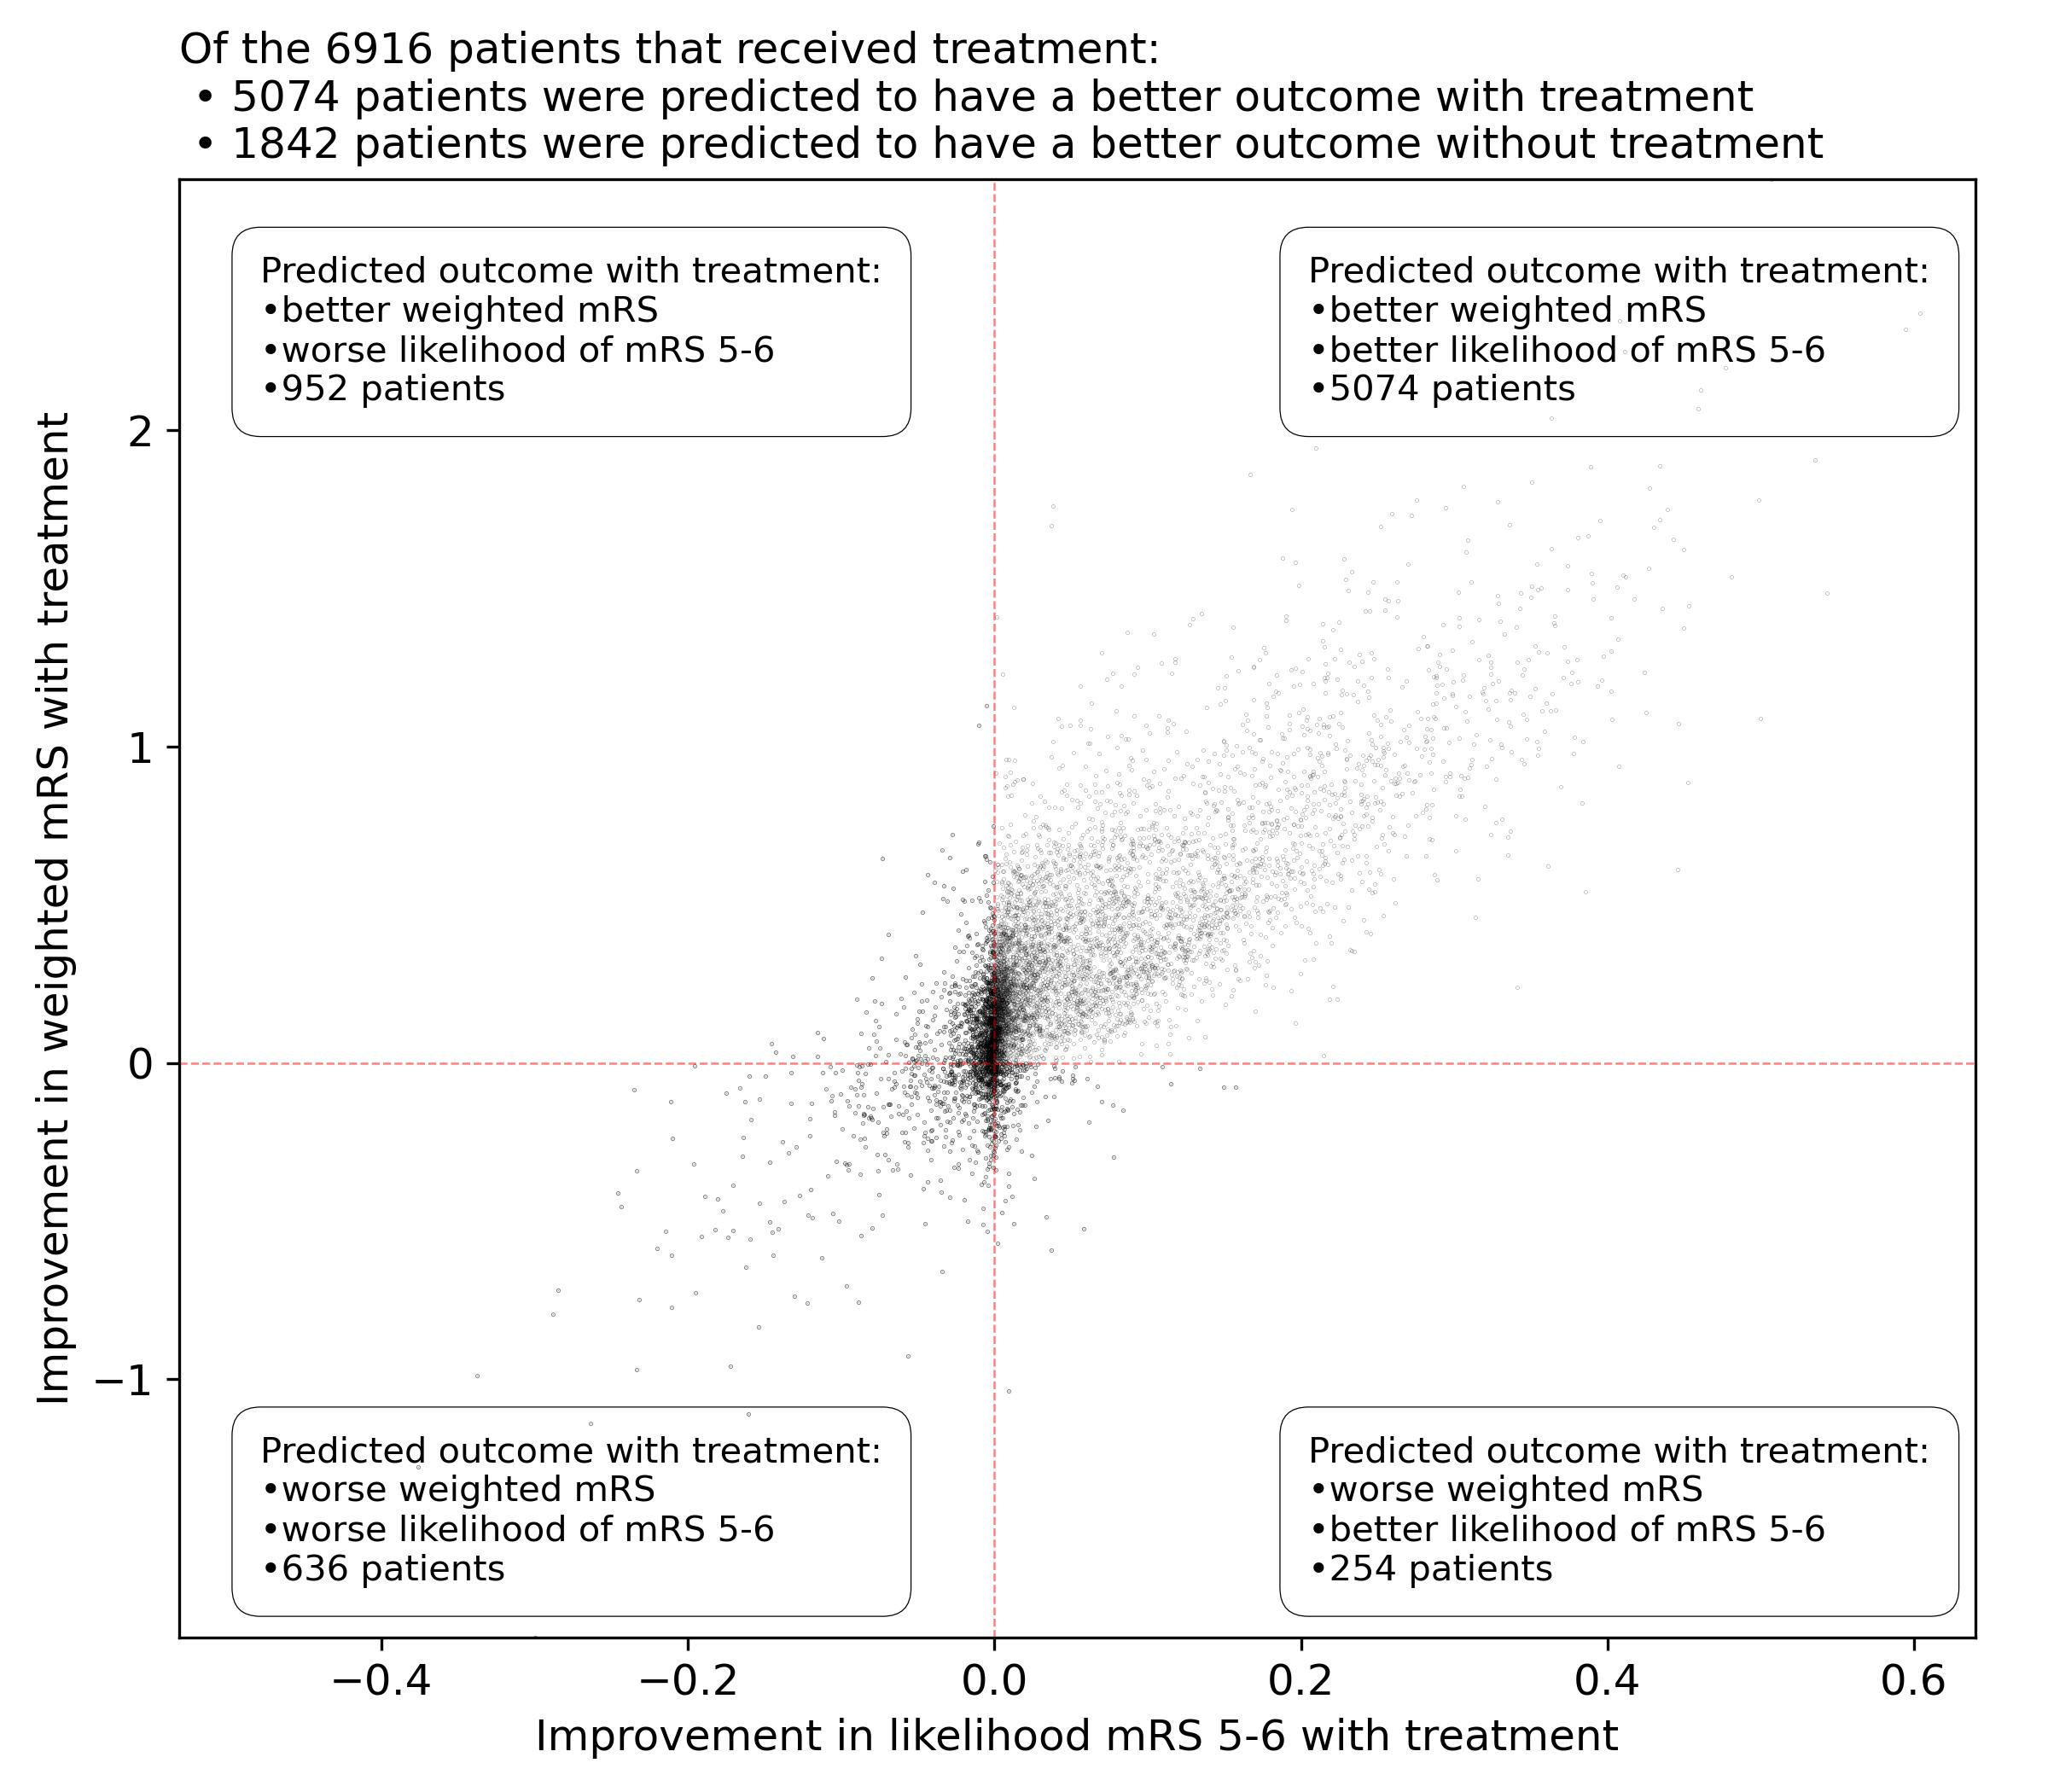
\includegraphics[trim={0 0 0 1.7cm}, clip, width=1\linewidth]{./images/p4_scatter_treated}
  \caption{\footnotesize{Patients who received thrombolysis}}
  \label{fig:scatter_receive}
\end{subfigure}

\vspace{5mm}


\begin{subfigure}{.7\textwidth}
  \centering
  \captionsetup{width=.9\linewidth}
  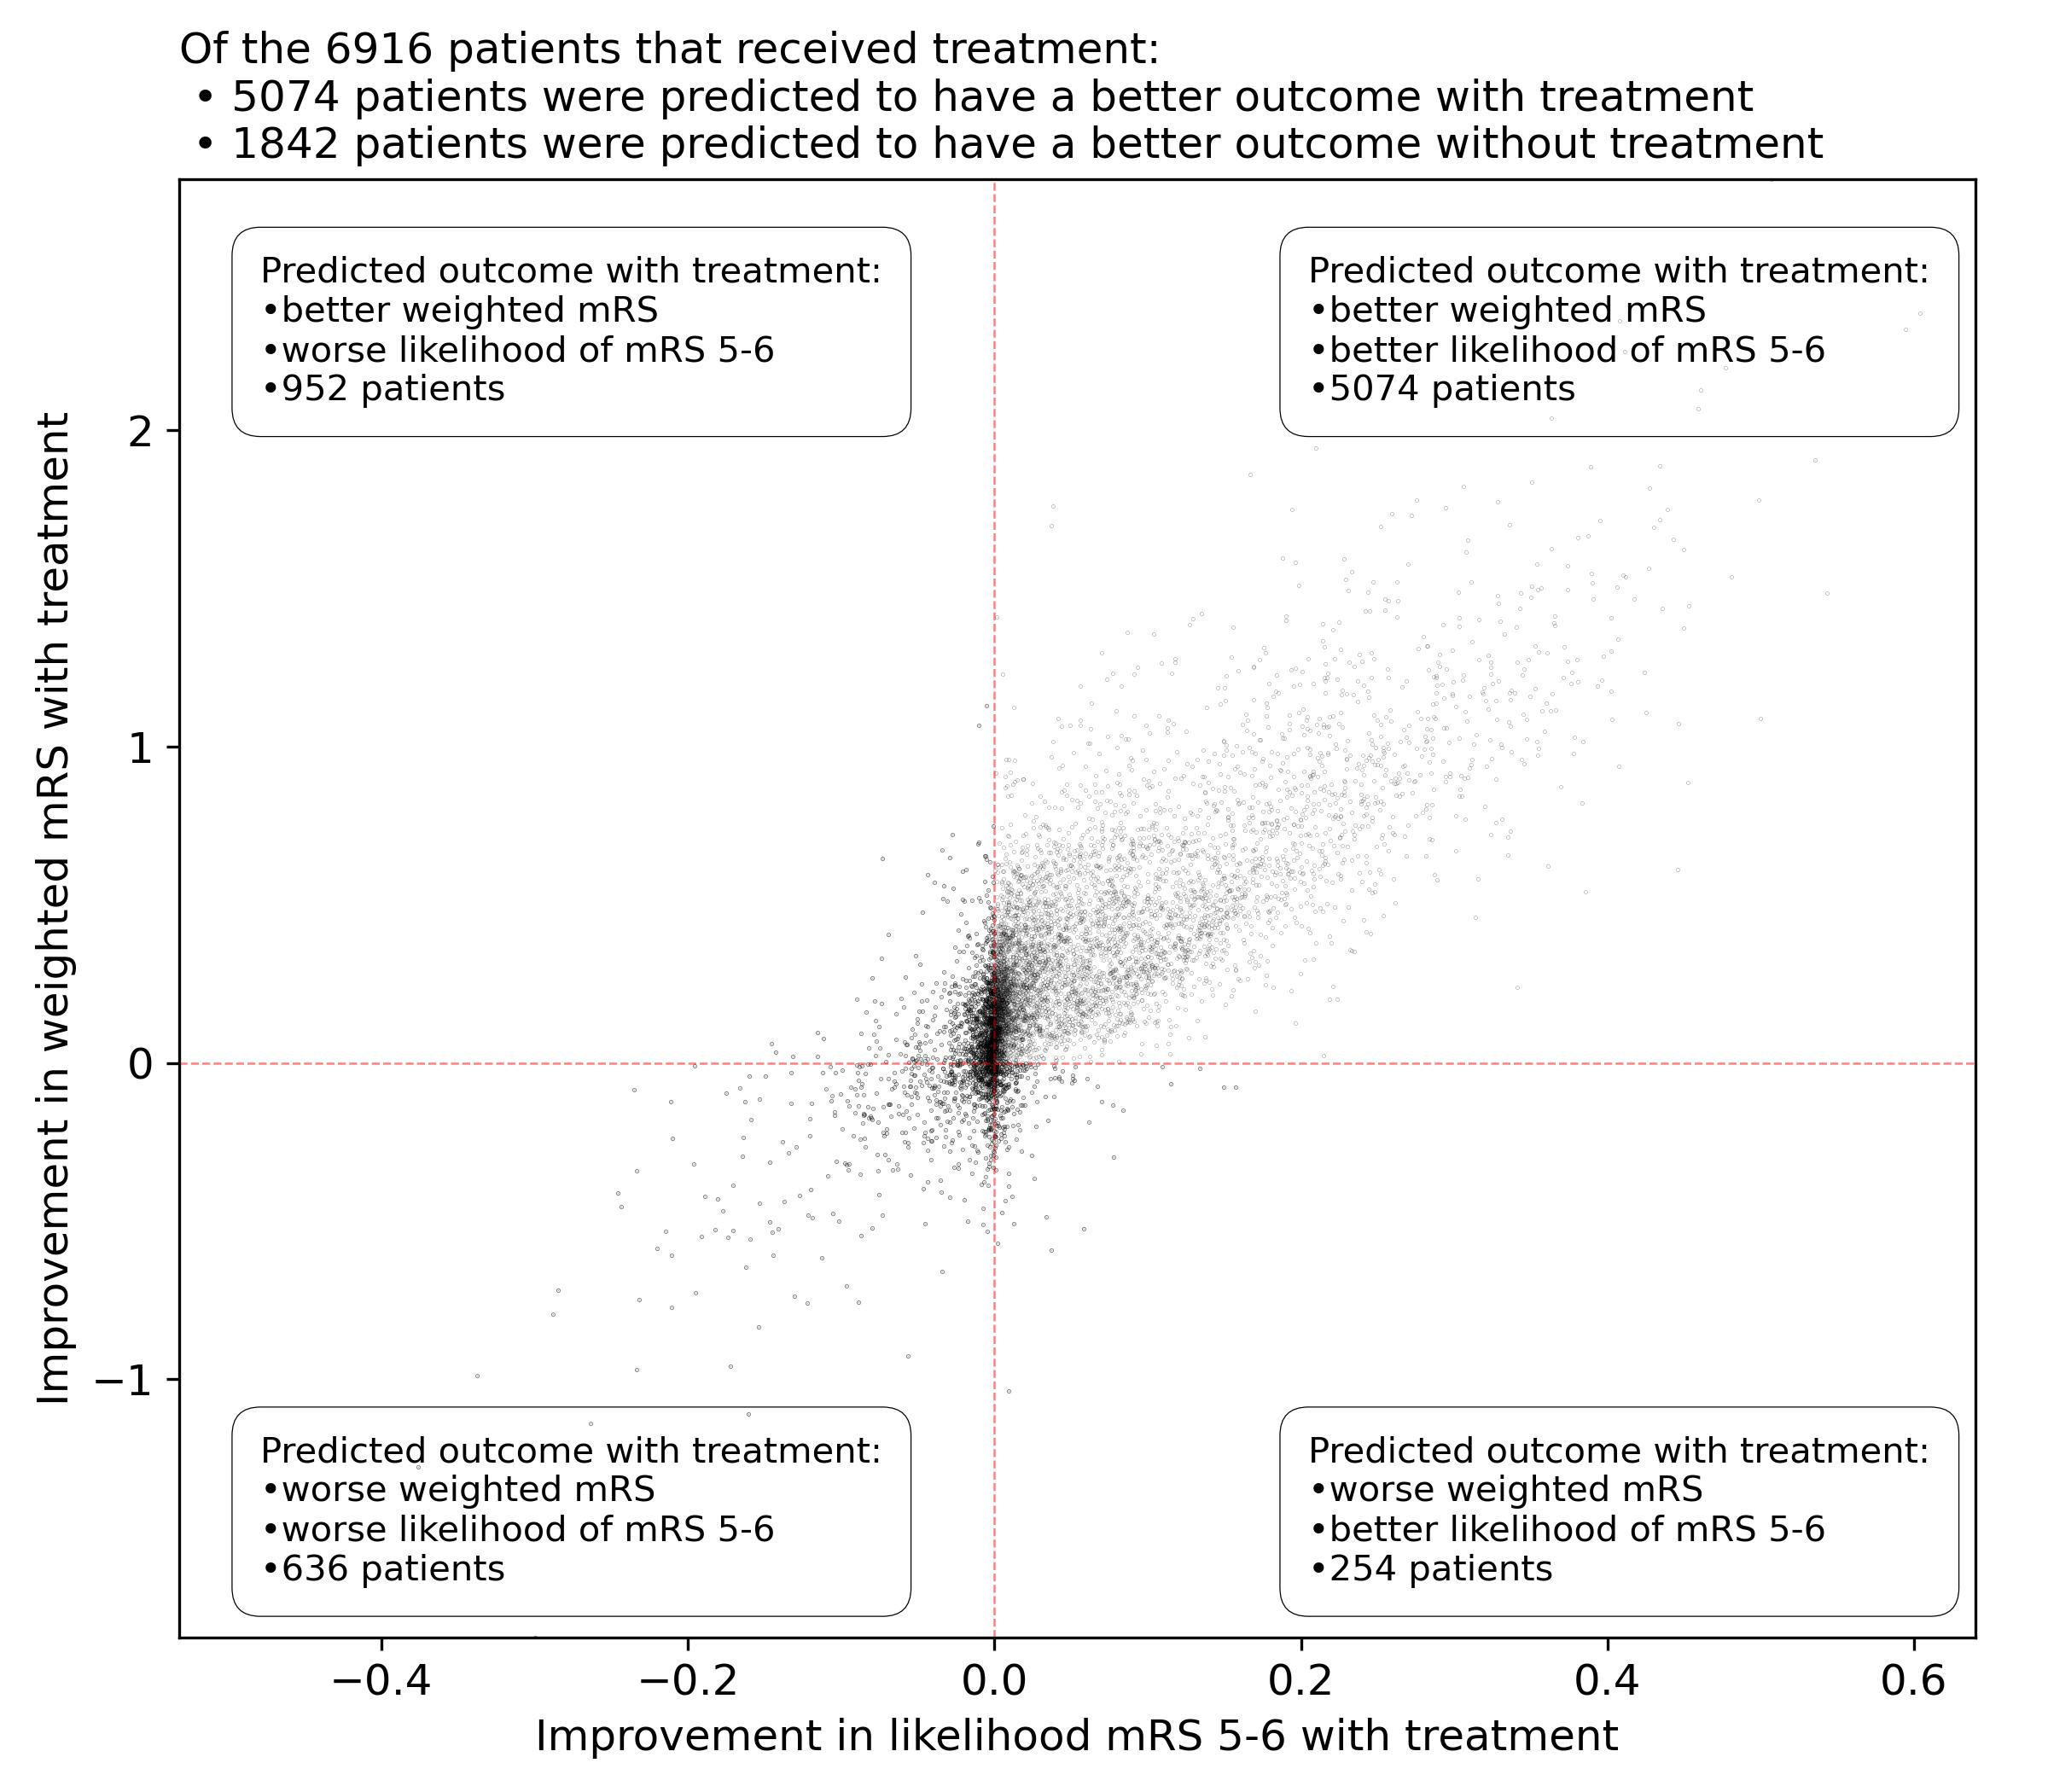
\includegraphics[trim={0 0 0 1.7cm}, clip, width=1\linewidth]{./images/p4_scatter_treated}
  \caption{\footnotesize{Patients who did not receive thrombolysis}}
  \label{fig:scatter_not_receive}
\end{subfigure}
  \caption{The predicted benefit or disbenefit of thrombolysis for each of 15,680 patients. Benefit is shown as both the expected improvement in probability-weighted disability (y-axis) and the improvement in likelihood of avoiding discharge with mRS 5-6. Both measures are expressed so that a positive value is better (a reduction in probability-weighted disability or a reduction in probability of discharge with mRS 5-6). (a) Patients who did actually receive thrombolysis, (b) Patients who did not actually receive thrombolysis.}
\label{fig:scatter_all}
\end{figure}

\subsection{Hospital trade-off between maximising benefit from thrombolysis and minimising risk of harm from thrombolysis}

The XGBoost \textit{thrombolysis decision} model had an accuracy of 78.7\% and ROC-AUC of 0.86. Figure \ref{fig:hosp_shap_scatter} shows the trade-off between the individuals hospital \textit{sensitivity} and \textit{specificity} towards giving treatment. We found that those hospitals attaining a higher predicted \textit{sensitivity} of treatment (not missing patients who would benefit from treatment) also tended to have a lower \textit{specificity} (giving thrombolysis to patients who would likely not benefit from it).

%218_hosp_shap_scatter.png}}\\

\begin{figure}
    \centering
    {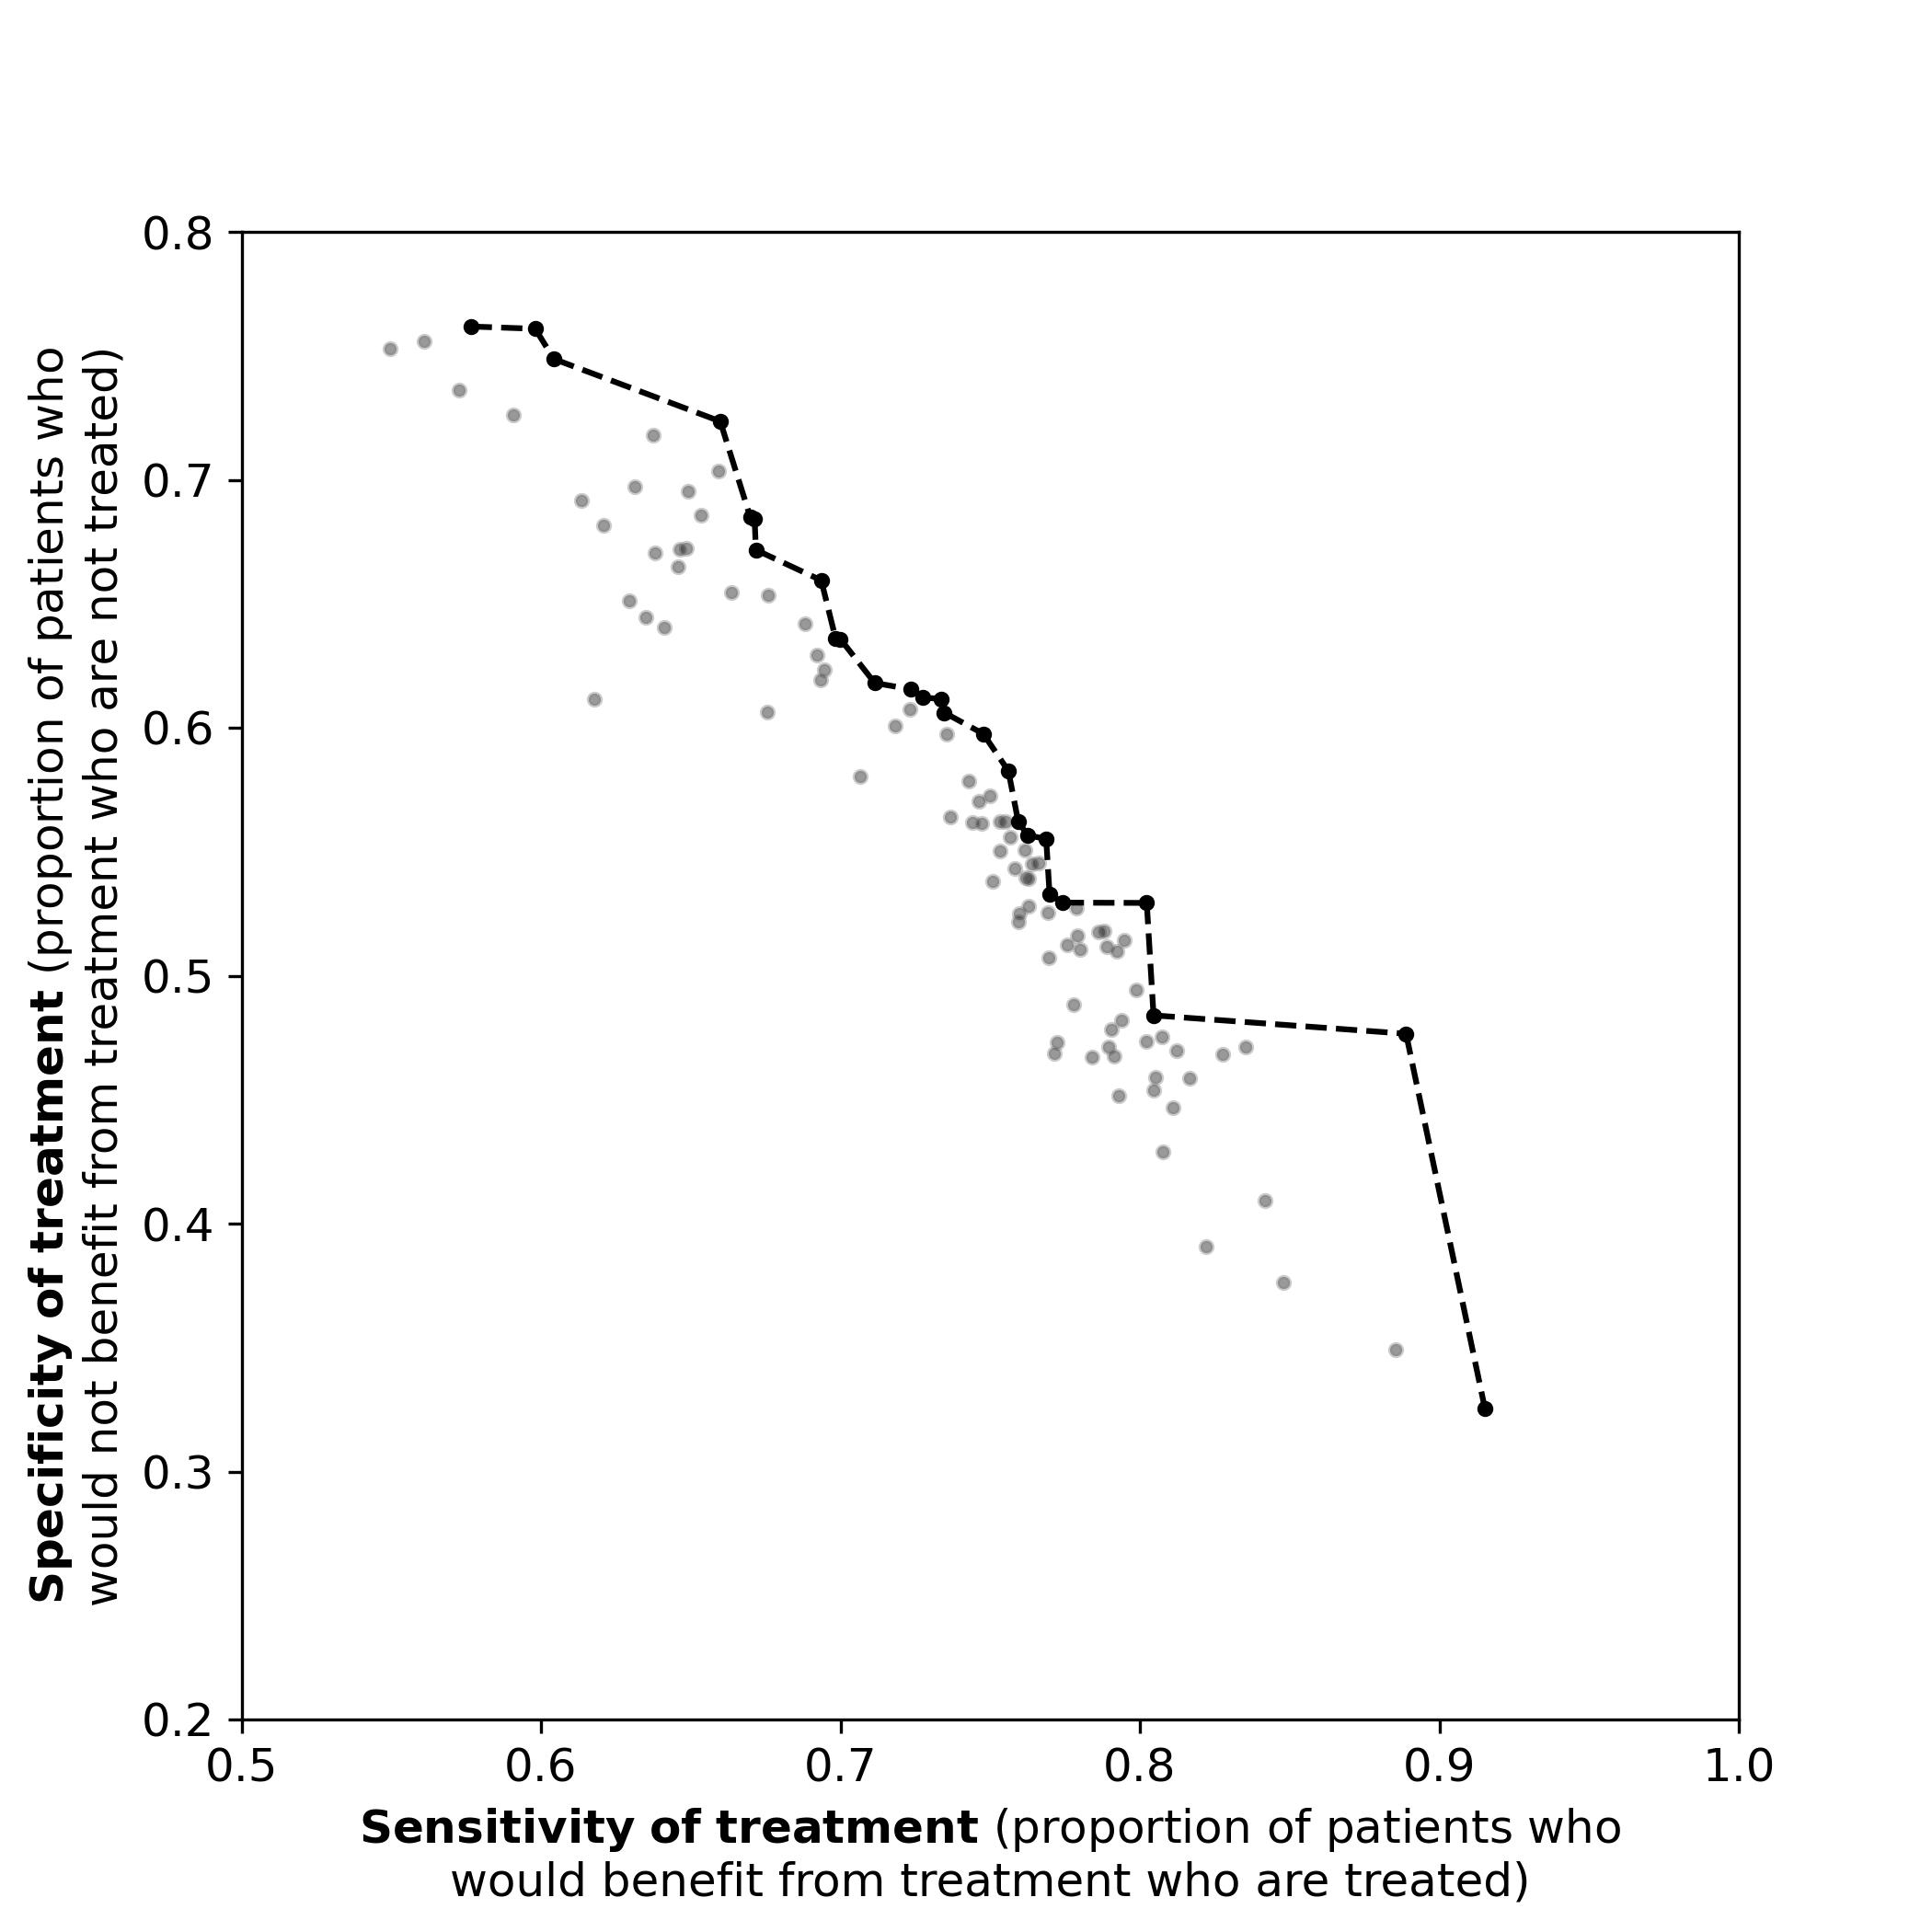
\includegraphics[width=0.75\linewidth]{./images/p4_spec_sens}} 
    \caption{\textit{Sensitivity} (proportion of patients who were predicted to benefit from thrombolysis who were predicted to receive thrombolysis) and \textit{specificity} (proportion of patients who were predicted \textit{not} to benefit from thrombolysis who were predicted \textit{not} to receive thrombolysis) for each stroke team. The dotted line shows the hospitals on the Pareto front where there are no hospitals that have a better \textit{sensitivity} without a worse \textit{specificity}, or vice-versa }
    \label{fig:hosp_shap_scatter}
\end{figure}

\subsection{Conclusions}

We found general agreement between actual thrombolysis use and best predicted outcomes, though we found decisions based on the outcome model would support higher use of thrombolysis than is actually the case. Of those who did not receive thrombolysis, the outcome model predicted that nearly half of them would have likely benefited from thrombolysis. Of those that did receive thrombolysis we found about one in four may be being given thrombolysis without there being predicted clear overall benefit. There was an apparent trade-off in decision-making between hospitals. Those hospitals who gave thrombolysis to more patients who would benefit from it (higher \textit{sensitivity}) were also more likely to give thrombolysis to more patients who would not benefit from it (lower \textit{specificity}). This represents a trade-off between `\textit{Miss no benefit}' and `\textit{Do no harm}'. Maximising benefit while minimising harm is likely to require more sophisticated guidance on use of thrombolysis, such as that indicated by our model.